\documentclass[oneside, 11pt]{article}

\usepackage[T1]{fontenc}
\usepackage[utf8]{inputenc}
\usepackage[english]{babel}

\usepackage{fouriernc}
\usepackage[detect-all, binary-units, separate-uncertainty=true,
            per-mode=symbol, retain-explicit-plus, retain-unity-mantissa=false]{siunitx}

\usepackage{setspace}
\setstretch{1.2}

\setlength{\parskip}{\smallskipamount}
\setlength{\parindent}{0pt}

\usepackage[headheight=14pt]{geometry}
\geometry{marginparwidth=0.5cm, verbose, a4paper, tmargin=3cm, bmargin=3cm,
          lmargin=2cm, rmargin=2cm}

\usepackage{float}

\usepackage[fleqn]{amsmath}
\numberwithin{equation}{section}
\numberwithin{figure}{section}

\usepackage{graphicx}
\graphicspath{{images/}{../../../images/}}

\usepackage{tikz}
\usetikzlibrary{shapes}
\usetikzlibrary{plotmarks}

\newcounter{Exercise}
\setcounter{Exercise}{1}
\usepackage{xcolor}
\definecolor{shadecolor}{gray}{0.9}
\usepackage{framed}
\usepackage{caption}

\usepackage{url}


\usepackage{fancyhdr}
\pagestyle{fancy}
\fancyhf{}
\rhead{\thepage}
\renewcommand{\footrulewidth}{0pt}
\renewcommand{\headrulewidth}{0pt}

\fancypagestyle{firststyle}
{
    \fancyhf{}
    \rhead{\thepage}
    \cfoot{
\includegraphics[height=30pt]{HiSPARClogo}}
    \rfoot{
\includegraphics[height=25pt]{CCbysa}}
    \lfoot{
\includegraphics[height=30pt]{NIKHEFlogo}}
    \renewcommand{\footskip}{50pt}
    \renewcommand{\footrulewidth}{0.1pt}
    \renewcommand{\headrulewidth}{0pt}
}

\newcommand{\figref}[1]{Figuur~\ref{#1}}

\newcommand{\hisparc}{\textsmaller{HiSPARC}\xspace}
\newcommand{\kascade}{\textsmaller{KASCADE}\xspace}
\newcommand{\sapphire}{\textsmaller{SAPPHiRE}\xspace}
\newcommand{\jsparc}{\textsmaller{jSparc}\xspace}
\newcommand{\hdf}{\textsmaller{HDF5}\xspace}
\newcommand{\aires}{\textsmaller{AIRES}\xspace}
\newcommand{\csv}{\textsmaller{CSV}\xspace}
\newcommand{\python}{\textsmaller{PYTHON}\xspace}
\newcommand{\corsika}{\textsmaller{CORSIKA}\xspace}
\newcommand{\labview}{\textsmaller{LabVIEW}\xspace}
\newcommand{\daq}{\textsmaller{DAQ}\xspace}
\newcommand{\adc}{\textsmaller{ADC}\xspace}
\newcommand{\hi}{\textsc{h i}\xspace}
\newcommand{\hii}{\textsc{h ii}\xspace}
\newcommand{\mip}{\textsmaller{MIP}\xspace}
\newcommand{\hisparcii}{\textsmaller{HiSPARC II}\xspace}
\newcommand{\hisparciii}{\textsmaller{HiSPARC III}\xspace}

\DeclareSIUnit{\electronvolt}{\ensuremath{\mathrm{e\!\!\:V}}}

\DeclareSIUnit{\unitsigma}{\ensuremath{\sigma}}
\DeclareSIUnit{\mip}{\textsmaller{MIP}}
\DeclareSIUnit{\adc}{\textsmaller{ADC}}

\DeclareSIUnit{\gauss}{G}
\DeclareSIUnit{\parsec}{pc}
\DeclareSIUnit{\year}{yr}



\begin{document}

\title{Kosmische Straling}
\author{N.G. Schultheiss}
\date{}

\maketitle
\thispagestyle{firststyle}

\section{Inleiding}

In de module ``De zon'' is te lezen dat de Zon zonnewind uitzendt.
Deze zonnewind valt uiteen in twee groepen. Een deel van de zonnewind
komt van de magnetische polen van de zon. Deze deeltjes hebben een
snelheid van ongeveer 400km/s. Een andere deel van de zonnewind komt
uit de zonnevlekken. Deze deeltjes hebben een snelheid van ongeveer
800km/s. Als we aannemen dat andere sterren zich op gelijke wijze
gedragen, komen hier ook deeltjes met vergelijkbare snelheden uit.

\begin{figure}[h]
\noindent \begin{centering}
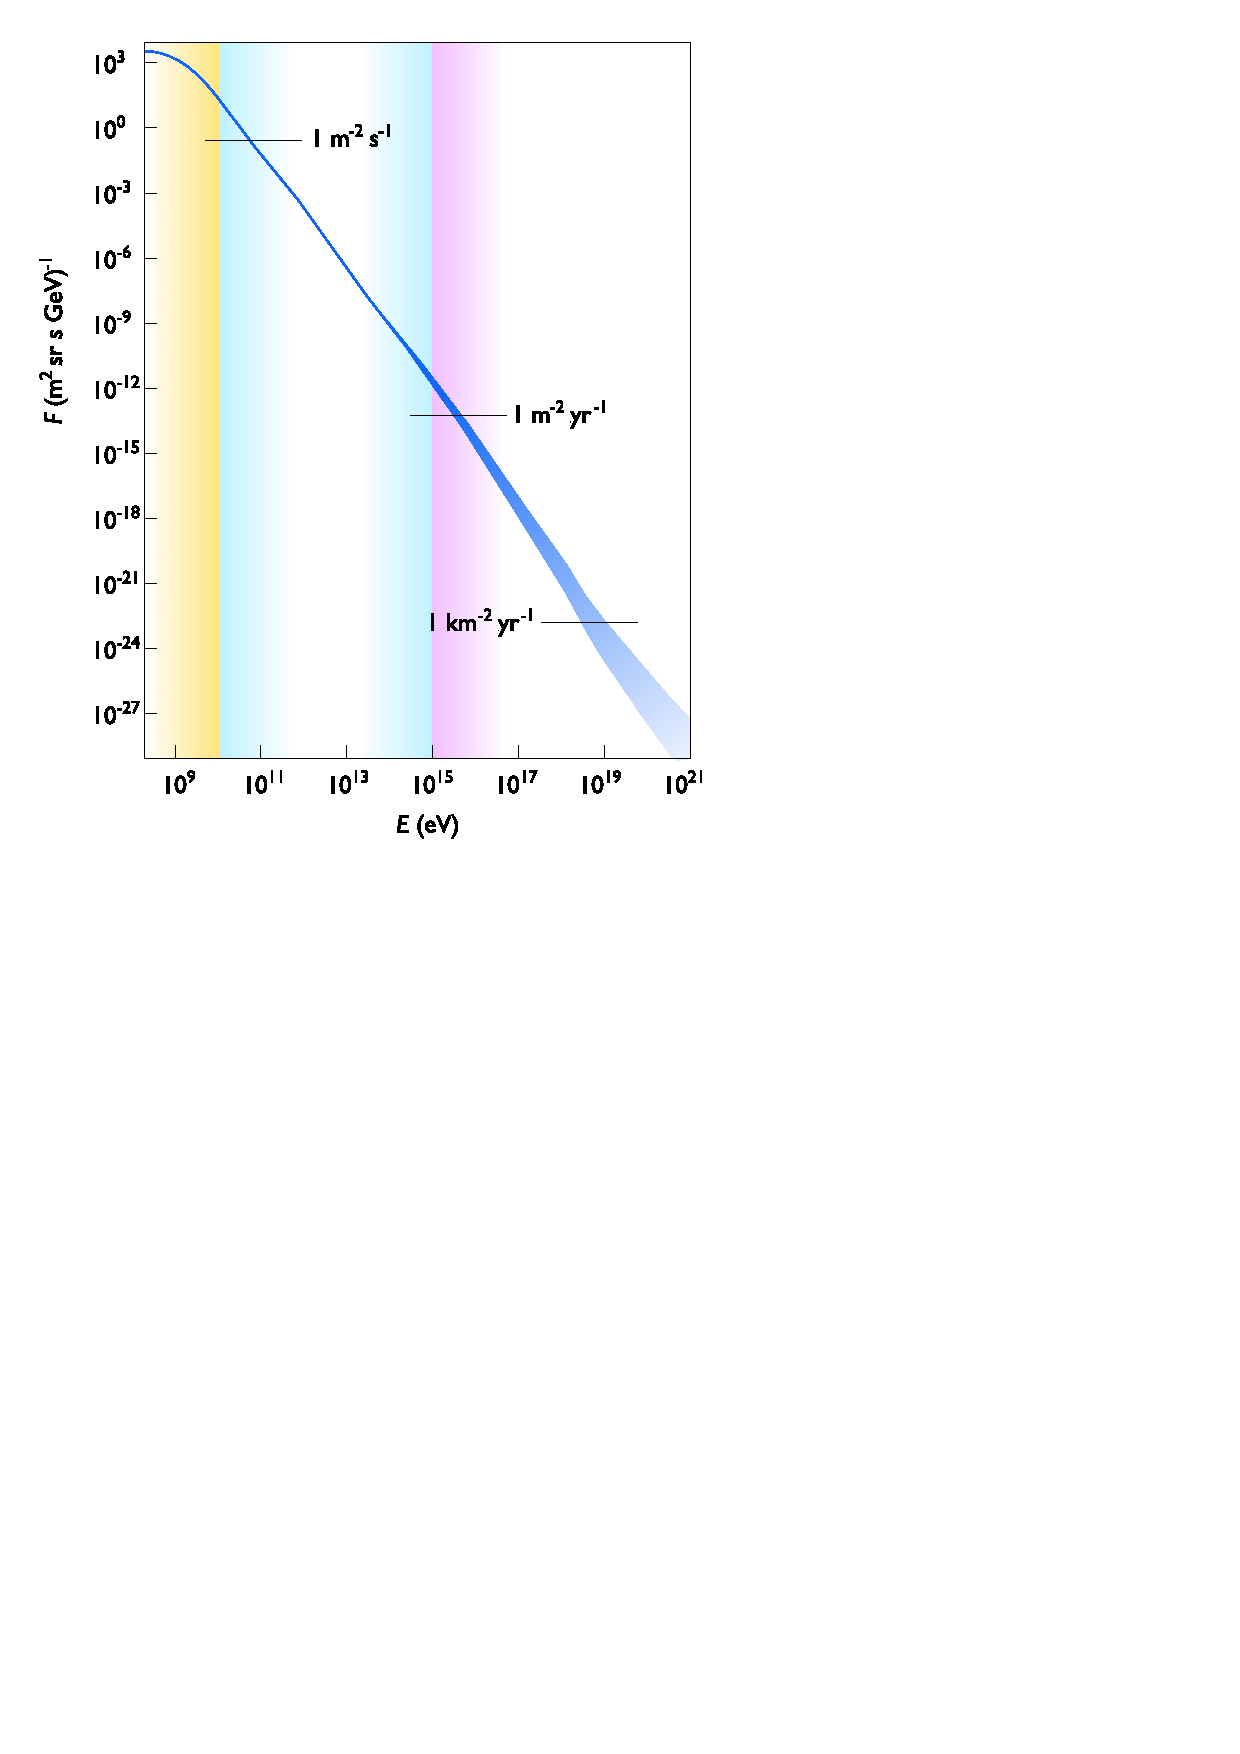
\includegraphics[scale=0.75]{Cosmic_ray_flux_versus_particle_energy}
\par\end{centering}

\caption{Kosmische straling\cite{cosmicrayflux}}
\end{figure}


Zoals in figuur 1.1 te zien is, is de gemeten energie van de kosmische
straling echter veel groter. Waar komt deze extra energie vandaan?


\section{Ladingen in magnetische velden}

Als een lading in een magnetisch veld beweegt ondervindt deze een
Lorentzkracht. In een divergerend veld zal de snelheid van de deeltjes
toenemen. Als er in het heelal een heel sterk divergerend veld is
zal de energie van de deeltjes die hier uitgezonden worden heel groot
worden. We kunnen dus op zoek gaan naar heftige kosmische verschijnselen
om figuur 1.1 te verklaren. Twee heftige verschijnselen zijn zwarte
gaten en supernova's.


\paragraph*{Opdracht 1:}

\emph{Wat kun je over de intensiteit van hoogenergetische kosmische
straling zeggen als deze afkomstig is van zwarte gaten? Wat is er
aan de hand als deze straling afkomstig is van supernova's? }

Gelukkig vinden supernova's ver van ons vandaan plaats. Als een nabijgelegen
ster een supernova wordt, betekent dit het einde van het leven op
Aarde en hoeven we dus verder geen onderzoek meer te doen. 

Stel dat we een proton met een energie van 100GeV detecteren en dat
deze afkomstig is van een supernova op een afstand van 100 lichtjaar.
Op kosmische schaal is dit vlakbij. Hoeveel eerder is het licht dan
bij ons als het proton?

Omdat de energie van het proton erg groot is, mogen we dit niet meer
oplossen met de formule $E=\frac{1}{2}mv^{2}$ maar moeten we $E=mc^{2}$
gebruiken. In de module ``Relativiteit'' wordt uitgelegd hoe deze
formule te gebruiken is. De formule wordt hier geschreven als $E=\gamma mc^{2}$,
hierin is de Lorentzconstante $\gamma=\frac{1}{\sqrt{1-\left(\frac{v}{c}\right)^{2}}}$.
In de Binas is te vinden dat de massa van een proton te schrijven
is als 938,3$\frac{\mathrm{MeV}}{c^{2}}$. Invullen geeft:

\begin{equation}
E=\frac{1}{\sqrt{1-\left(\frac{v}{c}\right)^{2}}}mc^{2}
\end{equation}


\begin{equation}
100\mathrm{GeV}=\frac{1}{\sqrt{1-\left(\frac{v}{c}\right)^{2}}}983,3\frac{\mathrm{MeV}}{c^{2}}c^{2}
\end{equation}


\begin{equation}
100\mathrm{GeV}=\frac{1}{\sqrt{1-\left(\frac{v}{c}\right)^{2}}}938,3\mathrm{MeV}
\end{equation}


\begin{equation}
\frac{100000}{938,3}=\frac{1}{\sqrt{1-\left(\frac{v}{c}\right)^{2}}}
\end{equation}


\begin{equation}
0,09669=1-\left(\frac{v}{c}\right)^{2}
\end{equation}


\begin{equation}
\left(\frac{v}{c}\right)^{2}=1-0,09669=0,90331
\end{equation}


\begin{equation}
\frac{v}{c}=0,95043
\end{equation}


\begin{equation}
v=0,95043c
\end{equation}


Het licht legt 100 lichtjaar in 100 jaar af. De protonen doen hier
$\frac{1}{0,95043}$ maal zo lang over. De protonen hebben dus $\frac{100}{0,95043}=105,22$jaar
nodig en komen ruim 5 jaar na het licht aan.


\paragraph*{Opdracht 2:}

\emph{Stel dat we protonen detecteren met een energie van 1000GeV.
Hoeveel later komen deze van de supernova op 100 lichtjaar aan?}


\section{Velden in de ruimte}

In de module ``Meten met telescopen'' is te lezen dat de Andromeda
nevel met een snelheid van 300 km/s naar ons toe komt. We kunnen aannemen
dat er in de Andromeda nevel magnetische velden zijn, deze komen ook
met 300km/s naar ons toe. Als een deeltje in een magnetisch veld komt,
ondervindt dit deeltje een Lorentzkracht.

\begin{figure}
\noindent \begin{centering}
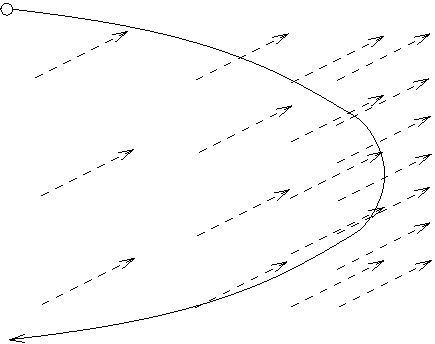
\includegraphics[scale=0.75]{veld1}
\par\end{centering}

\caption{Bewegende deeltjes in een stilstaand veld}
\end{figure}


Zoals te zien is, keert deeltje in het magnetisch veld om. Als de
Andromeda nevel op een stilstaand proton botst, krijgt het proton
op een vergelijkbare wijze een snelheid van 600km/s. Let op! Dit geldt
nu alleen omdat de snelheid van de Andromeda nevel ten opzicht van
de lichtsnelheid erg laag is. Als de snelheid hoger is moeten we de
botsing relativistisch berekenen. 

In hoofdstuk 2 hebben we het verschil in snelheid van protonen vergeleken
met de snelheid van fotonen (licht). Protonen ondervinden krachten
als ze door magnetische velden in de ruimte bewegen omfdat ze een
lading hebben. Bij fotonen, die geen lading hebben, is dit niet het
geval.


\paragraph*{Opdracht 3:}

\emph{Leg uit of het tijdsverschil tussen het licht uit een supernova
en de protonen uit een supernova groter of kleiner zal worden door
magnetische velden in de ruimte.}


\paragraph*{Opdracht 4:}

\emph{Leg uit of de richting van waaruit de deeltjes op Aarde komen
iets te maken heeft met de richting van de bron vanaf Aarde.}

Binnen het Melkwegstelsel zijn ook allerlei bewegende magnetische
velden te vinden, zoals bijvoorbeeld het veld van de Aarde. Als dit
veld op een geladen deeltje botst, zal dit deeltje ook versnellen.
Op deze manier kunnen er dus ook hoogenergetische deeltjes ontstaan.


\paragraph*{Opdracht 5:}

\emph{Beredeneer dat de kans op een botsing die deeltjes versneld
groter, evengroot of kleiner is dan de kans op een botsing die deeltjes
vertraagd.}


\paragraph*{Opdracht 6:}

\emph{Als de Andromeda nevel recht naar het melkwegstelsel komt, zullen
ze vroeg of laat botsen. Leg uit dat bij een dergelijke botsing veel
snelle geladen deeltjes vrijkomen.}


\begin{thebibliography}{9}
    \bibitem{cosmicrayflux}
        Door Sven Lafebre (naar Swordy), \emph{Cosmic ray flux versus particle energy}, CC-BY-SA-3.0, via Wikimedia Commons
\end{thebibliography}

\end{document}
